\documentclass[a4paper]{article}
\usepackage{vntex}
\usepackage[english]{babel}
\usepackage[utf8]{inputenc}

\usepackage[table]{xcolor}
\definecolor{lightgray}{gray}{0.9}
\definecolor{atomictangerine}{rgb}{1.0, 0.6, 0.4}
\usepackage[utf8]{inputenc}
%\usepackage[francais]{babel}
\usepackage{a4wide}
\usepackage{amssymb}
\usepackage{epsfig}
\usepackage{latexsym}
\usepackage{multicol}
\usepackage{array}
\usepackage{hhline}
\usepackage{fancyhdr}
\usepackage{amsmath}
\usepackage{lastpage}
\usepackage[lined,boxed,commentsnumbered]{algorithm2e}
\usepackage{enumerate}
\usepackage{color}
\usepackage{graphicx}							% Standard graphics package
\usepackage{array}
\usepackage{tabularx, caption}
\usepackage{multirow}
\usepackage{multicol}
\usepackage{rotating}
\usepackage{graphics}
\usepackage{geometry}
\usepackage{setspace}
\usepackage{epsfig}
\usepackage{tikz}
\usepackage{verbatim}
\usepackage{cprotect}
\usetikzlibrary{arrows,snakes,backgrounds}
\usepackage{hyperref}
\usepackage{listings}
\hypersetup{urlcolor=blue,linkcolor=black,citecolor=black,colorlinks=true} 
%\usepackage{pstcol} 								% PSTricks with the standard color package

%\usepackage{fancyhdr}
\setlength{\headheight}{40pt}
\setlength{\extrarowheight}{3.5pt}
\pagestyle{fancy}
\fancyhead{} % clear all header fields
\fancyhead[L]{
 \begin{tabular}{rl}
    \begin{picture}(25,15)(0,0)
    \put(0,-8){
\includegraphics[width=8mm, height=8mm]{img/hcmut.png}}
    %\put(0,-8){\epsfig{width=10mm,figure=hcmut.eps}}
   \end{picture}&
	%
\includegraphics[width=8mm, height=8mm]{hcmut.png} & %
	\begin{tabular}{l}
		\textbf{\bf \ttfamily {\color{blue}Ho Chi Minh City University of Technology}}\\
		\textbf{\bf \ttfamily {\color{blue}Falcuty of Computer Science and Engineering}}
	\end{tabular} 	
 \end{tabular}
}
\fancyhead[R]{
	\begin{tabular}{l}
		\tiny \bf \\
		\tiny \bf 
	\end{tabular}  }
\fancyfoot{} % clear all footer fields
\fancyfoot[L]{\scriptsize \ttfamily Project, The course on Probability and Statistics (MT2001) -- 2020/2021}
\fancyfoot[R]{\scriptsize \ttfamily Page {\thepage}/\pageref{LastPage}}
\renewcommand{\headrulewidth}{0.3pt}
\renewcommand{\footrulewidth}{0.3pt}


%%%
\setcounter{secnumdepth}{4}
\setcounter{tocdepth}{3}
\makeatletter
\newcounter {subsubsubsection}[subsubsection]
\renewcommand\thesubsubsubsection{\thesubsubsection .\@alph\c@subsubsubsection}
\newcommand\subsubsubsection{\@startsection{subsubsubsection}{4}{\z@}%
                                     {-3.25ex\@plus -1ex \@minus -.2ex}%
                                     {1.5ex \@plus .2ex}%
                                     {\normalfont\normalsize\bfseries}}
\newcommand*\l@subsubsubsection{\@dottedtocline{3}{10.0em}{4.1em}}
\newcommand*{\subsubsubsectionmark}[1]{}
\makeatother


\begin{document}

\begin{titlepage}
\begin{center}
VIETNAM NATIONAL UNIVERSITY - HCM \\
Ho Chi Minh City University of Technology \\
Faculty of Computer Science and Engineering 
\end{center}

\vspace{1cm}

\begin{figure}[h!]
\begin{center}

\includegraphics[width=5cm]{img/hcmut.png}
\end{center}
\end{figure}

\vspace{1cm}


\begin{center}
\begin{tabular}{c}
\multicolumn{1}{l}{\textbf{{\Large {\color{blue}PROBABILITY AND STATISTICS (MT2001)}}}}\\
~~\\
\hline
\\
\multicolumn{1}{l}{\textbf{{\Large {\color{blue}Project Report: }}}}\\
\\
\textbf{{\Huge {\color{blue}Data Analysis}}}\\
\\
\hline
\end{tabular}
\end{center}

\vspace{1.5cm}

\begin{table}[h]
\begin{tabular}{rrl}
\hspace{7 cm} &Instructor: & Mr. Nguyễn Tiến Dũng \\
& Students: & Ôn Quân An - 1852221 \\
& & Lê Thiên Ân - 1852255 \\
& & Trần Quốc Anh - 1852247 \\
& & Đào Đức Bảo - 1852258 \\
\end{tabular}
\end{table}
\vspace{1.7cm}
\begin{center}
{\footnotesize Ho Chi Minh City, June 2020}
\end{center}
\end{titlepage}


%\thispagestyle{empty}
\newpage
\renewcommand*\contentsname{Contents}
\tableofcontents
\newpage
\lstdefinestyle{mystyle}{   
    keywordstyle=\color{magenta},
    basicstyle=\ttfamily\footnotesize,
    breakatwhitespace=false,         
    breaklines=true,                 
    captionpos=b,                    
    keepspaces=true,                 
    numbers=left,                    
    numbersep=5pt,                  
    showspaces=false,                
    showstringspaces=false,
    showtabs=false,                  
    tabsize=2,
    frame=single,
}

\lstset{style=mystyle}



%%%%%%%%%%%%%%%%%%%%%%%%%%%%%%%%%
\section{Dataset Description}
{\Large \textbf{Medical Cost Personal Datasets}}
\begin{itemize}
    \item This Data is practically is used in the book “Machine Learning with R by Brett Lantz”; which is a book that provides an introduction to machine learning using R.\\ ({\color{blue}https://www.amazon.com/Machine-Learning-R-Brett-Lantz/dp/1782162143}).
    \item All of these datasets are in the public domain but simply needed some cleaning up and recoding to match the format in the book. The following data obtained from Kaggle, explain the cost of a small sample of US population Medical Insurance Cost based on some attributes depicted below.
\end{itemize}
\begin{center} 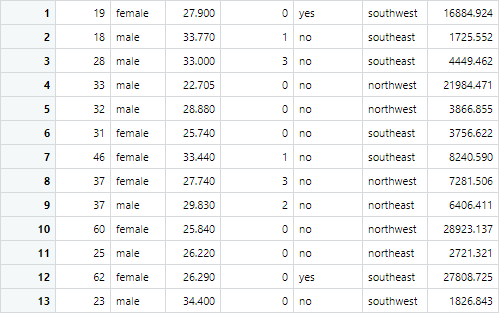
\includegraphics[width=13cm]{img/dataset.png} \\ (1325 rows remaining)\end{center}
{\large \textbf{Content of dataset:}}
 \begin{itemize}
     \item \textbf{age}: age of primary beneficiary
     \item \textbf{sex}: insurance contractor gender, [female, male]
     \item \textbf{bmi}: Body mass index, providing an understanding of body, weights that are relatively high or low relative to height, objective index of body weight (kg / $m^2$) using the ratio of height to weight.
     \item \textbf{children}: Number of children covered by health insurance / Number of dependents
     \item \textbf{smoker}: Smoking, [yes, no]
     \item \textbf{region}: the beneficiary's residential area in the US, [northeast, southeast, southwest, northwest]
     \item \textbf{charges}: Individual medical costs billed by health insurance
 \end{itemize}
{\large \textbf{Type of attributes:}}
 \begin{itemize}
     \item “\textbf{age}” is ordinal, “\textbf{sex}” is categorical, “\textbf{bmi}” is quantitative, “\textbf{children}” is quantitative, “\textbf{smoker}” is categorical, “\textbf{region}” is categorical, “\textbf{charges}” is quantitative.
 \end{itemize}


%%%%%%%%%%%%%%%%%%%%%%%%%%%%%%%%%

\section{Statistical Method}
\subsection{Linear Regression}
\subsubsection{Definition}
In statistics, \textbf{linear regression} is a linear approach to modeling the relationship between a scalar response (or dependent variable) and one or more explanatory variables (or independent variables). The case of one explanatory variable is called simple linear regression. For more than one explanatory variable, the process is called \textbf{multiple linear regression}. This term is distinct from multivariate linear regression, where multiple correlated dependent variables are predicted, rather than a single scalar variable.
\subsubsection{Exploratory Data Analysis}
The dataset depicts information about a person which is categorized into seven categories including \textbf{age}, \textbf{sex}, \textbf{BMI}, \textbf{children}, \textbf{smoker}, \textbf{region} and \textbf{charges}. After going through the dataset for some times, we concluded that it is rather reasonable to assume that the variable charges is influenced by the rest six variables. Therefore, we are going to check if the dataset is a suitable candidate for the Linear Regression data analysis method and if our assumption is satisfiable. \\ \\
Initially, we need to check the correlation between our targeted variable (\textbf{charges}) and the other independent variables (\textbf{age}, \textbf{sex}, \textbf{BMI}, \textbf{children}, \textbf{smoker}, \textbf{region}).
\newpage
\begin{center}
    \textbf{Correlation between Charges and Age/BMI/Children/Smoker/Region} \\
    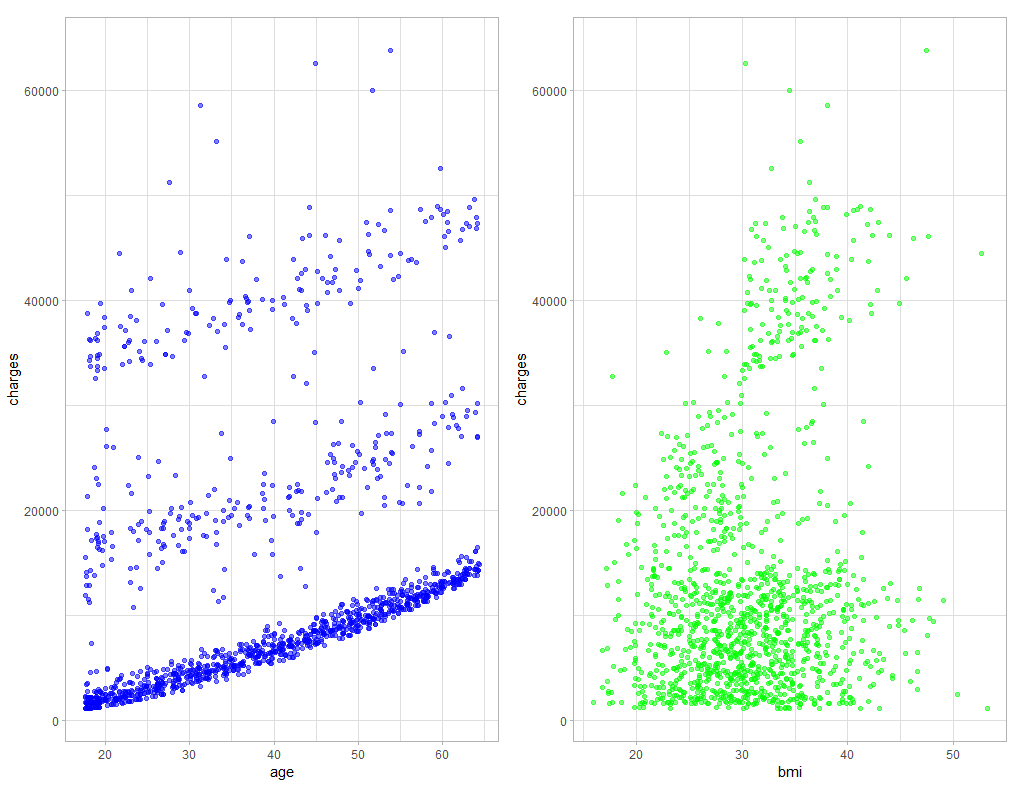
\includegraphics[width=12cm]{img/plot1.png} \\
    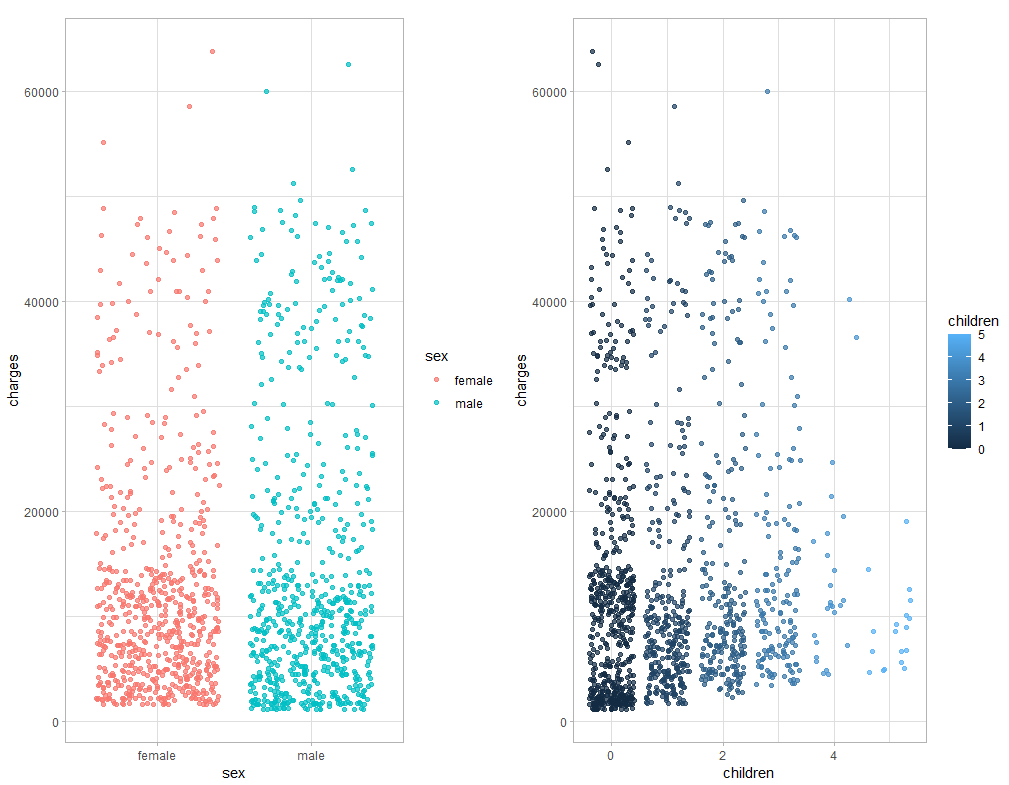
\includegraphics[width=13cm]{img/plot2.png} \\
    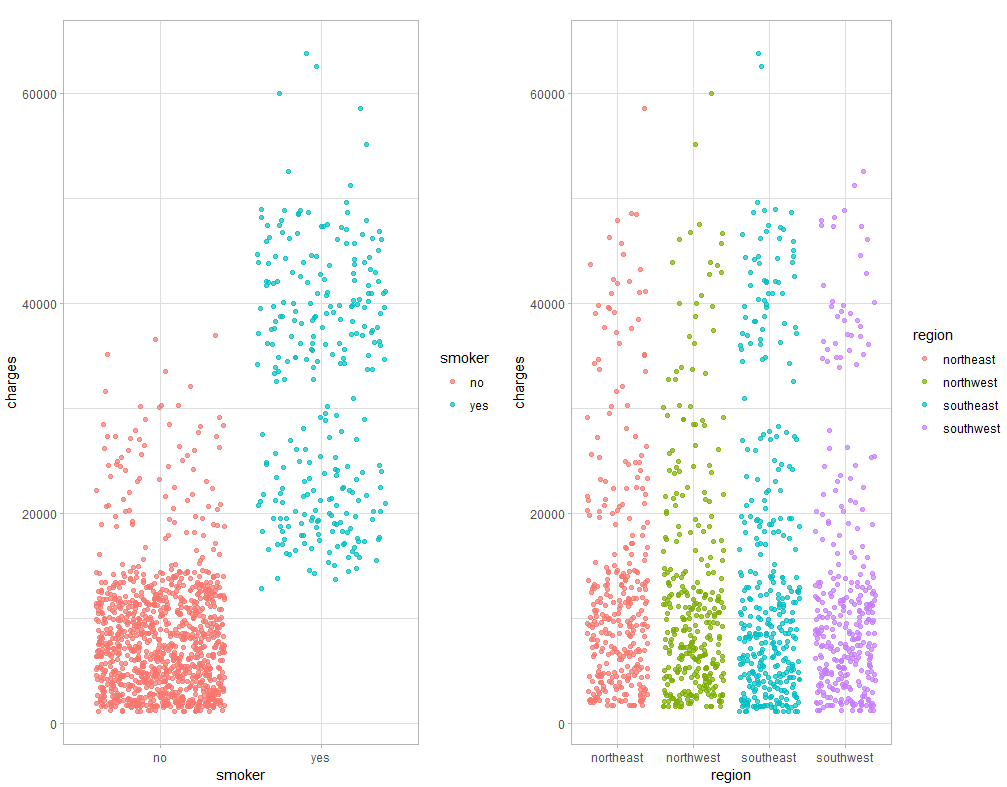
\includegraphics[width=13cm]{img/plot3.png}
\end{center}
\textbf{Summary:}
\begin{enumerate}
    \item As Age and BMI go up Charges for health insurance also trends up.
    \item No obvious connection between Charges and Sex. Charges for insurance with 4-5 children covered seems to go down.
    \item Charges for Smokers are higher than non-smokers. No obvious connection between Charges and Region.
\end{enumerate}
\subsubsection{Implementation}

\textbf{Hypothesis representation}: \\ \\
We will use $x_i$ to denote the independent variable and $y_i$ to denote dependent variable. For Simple Linear regression, a pair of ($x_i$,$y_i$) is called training example. The subscript i in the notation is simply index into the training set. We have m training example then i=1,2,3,...m. \\
The hypothesis function represented as:
\begin{center}
    $h_\theta$($x_i$) = $\theta_0$ + $\theta_1$*$x_i$
\end{center}
\begin{itemize}
    \item $\theta_0$, $\theta_1$ are parameters of hypothesis
\end{itemize}
However, as our assumption suggests, the target variables will presumably be influenced by the other six variables. Hence, applying Simpler Linear Regression on this dataset will not be satisfiable for the data analysis process as well as forecasting the possible trend. \\ \\
To tackle this, we will be adopting a more advanced and reliable method, namely, Multiple Linear Regression method. In this method, we will denote the independent variables by $x_i$ and $y_i$ will be the dependent variable. We have n independent variable then j = 1,2,3...n. 
\begin{center}
    $h_\theta$($x_i$) = $\theta_0$ + $\theta_1$*$x_{i1}$ + $\theta_2$*$x_{i2}$ + . . . + $\theta_j$*$x_{ij}$ + . . . + $\theta_n$*$x_{mn}$
\end{center}
\begin{itemize}
    \item $\theta_0$, $\theta_1$, ... , $\theta_j$….$\theta_n$ are parameter of hypothesis.
    \item m Number of training examples.
    \item n Number of independent variables.
    \item $x_{ij}$ is $i^{th}$ training example of $j^{th}$ feature.
\end{itemize}
Now for the real work. To judge how how good our model is, we need something to test it against. We can accomplish this using a technique called cross-validation. Cross-validation can get much more complicated and powerful, but in this example, due to being inexperienced as well as to avoid undesirable errors, we are going do the most simple version of this technique. \\
\textbf{Steps}:
\begin{enumerate}
    \item Divide the dataset into two datasets: A ‘training’ dataset that we will use to train our model and a ‘test’ dataset that we will use to judge the accuracy of that model.
    \item Train the model on the ‘training’ data.
    \item Apply that model to the test data’s X variable, creating the model’s guesses for the test data’s Ys.
    \item Compare how close the model’s predictions for the test data’s Ys were to the actual test data Ys.
\end{enumerate}
Separating data into training and testing sets is an important part of evaluating data mining models. Typically, when we separate a data set into a training set and testing set, most of the data is used for training, and a smaller portion of the data is used for testing. With these step, we can avoid problems like overfitting. \\ \\
\textbf{Splitting the Data} \\
Here, we divide the dataset into two parts, 70\% random data for training and 30\% left for testing.
\begin{lstlisting}
split <- sample.split(data, SplitRatio = 0.7)
Data_train <- subset(data, split = "TRUE")
Data_test <- subset(data, split = "FALSE")
\end{lstlisting}
\textbf{Train the Model} \\
There are seven independent variables. The target variable here is \textbf{charges} and remaining six variables: \textbf{age}, \textbf{sex}, \textbf{bmi}, \textbf{children}, \textbf{smoker}, \textbf{region} are independent variable. There are multiple independent variables, so we need to fit Multiple linear regression. Then the hypothesis function should looks like:
\begin{center}
    $h_\theta$($x_i$) = $\theta_0$ + $\theta_1$*age + $\theta_2$*sex + $\theta_3$*bmi + $\theta_4$*children + $\theta_5$*smoker + $\theta_6$*region
\end{center}
In order to forecast the possible values for the dependent variable, we will be using our model parameter for the train dataset. Thereafter, comparisons between the model and the actual value in test set will be made. We compute \textbf{Mean Square Error} using formula:
\begin{center}
    J($\theta$) = $\frac{1}{m}$ $\sum_{i=1}^{m}$ $(\hat{y_i} - y_i)^{2}$
\end{center}
$R^2$ is statistical measure of how close data are to the fitted regression line. $R^2$ is always between 0 to 1. 0 indicated that model explains none of the variability of the response data around it's mean. 1 indicated that model explains all the variability of the response data around the mean.
\begin{center}
    $R^2$ = 1 - $\frac{SSE}{SST}$
\end{center}
\begin{center}
    SSE (Sum of Square Error) = $\sum_{i=1}^{m}$ $(\hat{y_i} - y_i)^{2}$
\end{center}
\begin{center}
    SST (Sum of Square Total) = $\sum_{i=1}^{m}$ $(y_i - \bar{y_i})^{2}$
\end{center}
But RStudio has provided us with an excellent and simple-to-use function to calculate these things:
\begin{lstlisting}
formula_0 <- as.formula("charges ~ age + sex + bmi + children + smoker + region)
model_0 <- lm(formula_0, data = Data_train)
\end{lstlisting}
We then get the summary of the created model.
\begin{center}
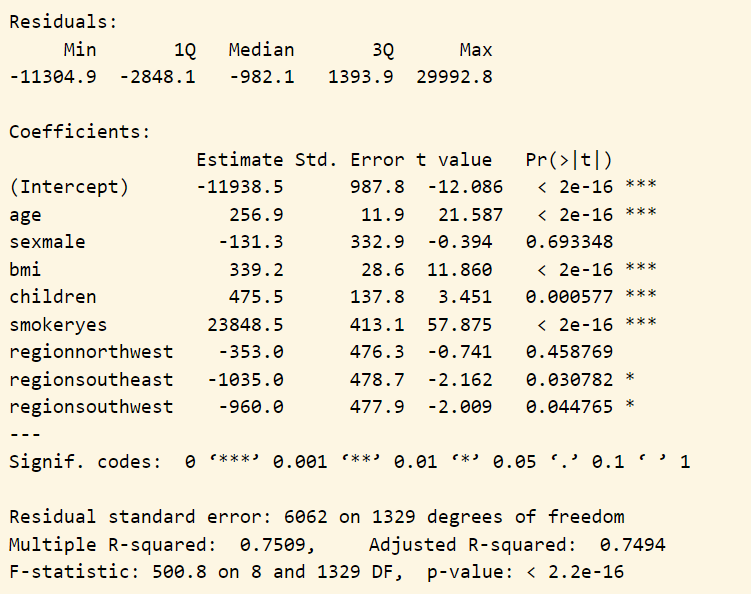
\includegraphics[width=14cm]{img/summary.png}
\end{center}
According to the summary, it is evident that smoking seems to have a great influence on the \textbf{charges} whereas \textbf{sex} does not leave much impact on the cost. From this information, we can conclude that the dataset is a potential candidate for Linear Regression. Hence, to simplify the problem, we will then create another model without the non-significant variables and check if the performance can be improved. Ultimately, we have the new simplified model which has only \textbf{age}, \textbf{bmi}, \textbf{children}, \textbf{region} and \textbf{smoker}.
\begin{lstlisting}
formula_1 <- as.formula("charges ~ age + bmi + children + smoker + region)
model_1 <- lm(formula_1, data = Data_train)
\end{lstlisting}
We then compare the new model with the original one.
\begin{itemize}
    \item Adjusted R-squared for first model: 0.7494
    \item Adjusted R-squared for second model: 0.7496
    \item RMSE for first model: 6041.68
    \item RMSE for second model: 6042.03
\end{itemize}
As we can see, the performance of the second model does not differ much from the original model. Hence, we will use the second model since it is simpler.
\subsubsection{Model Performance}
Now that we have trained the model, to determine the predicting performance of the trained model, comparisons with the test data will be made.
\begin{center}
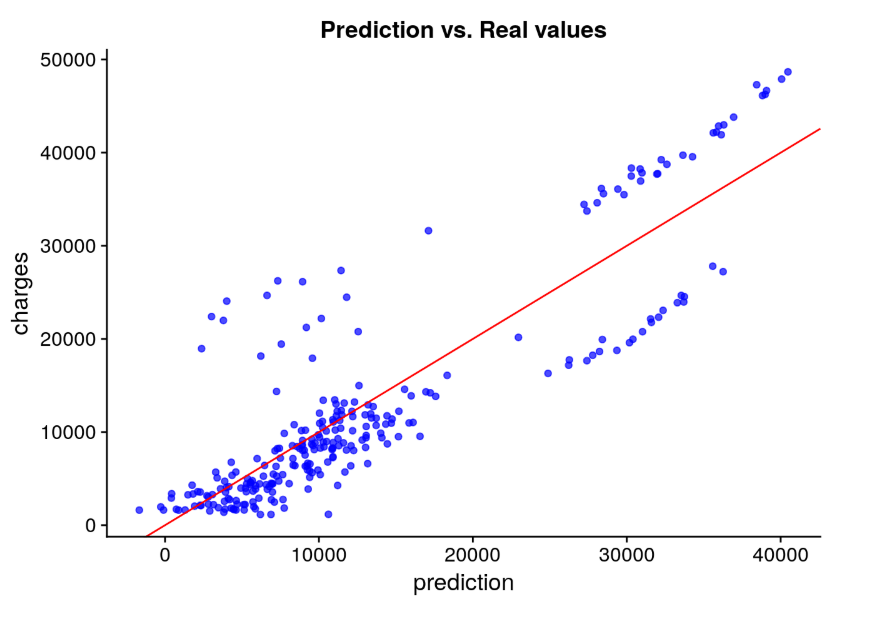
\includegraphics[width=8cm]{img/1.png}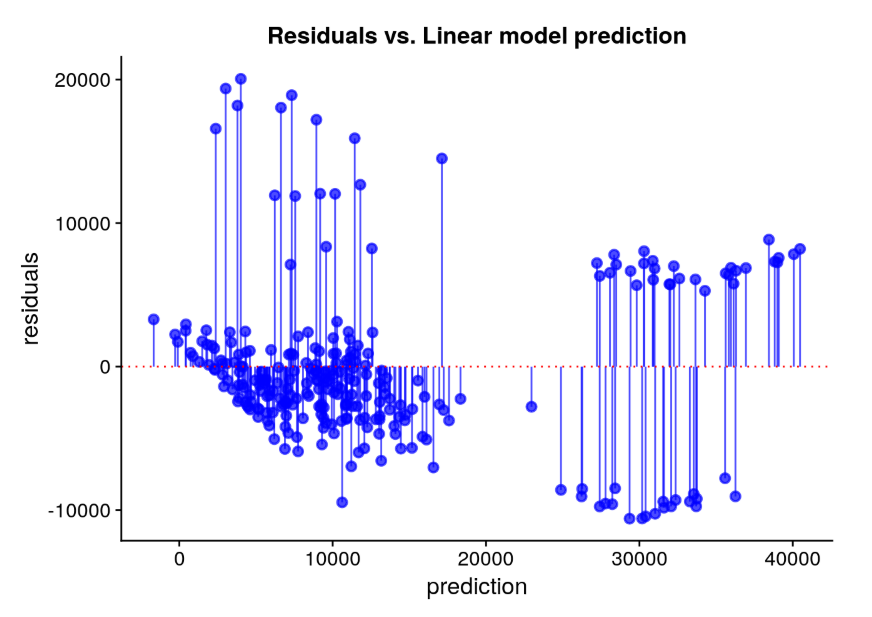
\includegraphics[width=8cm]{img/2.png}
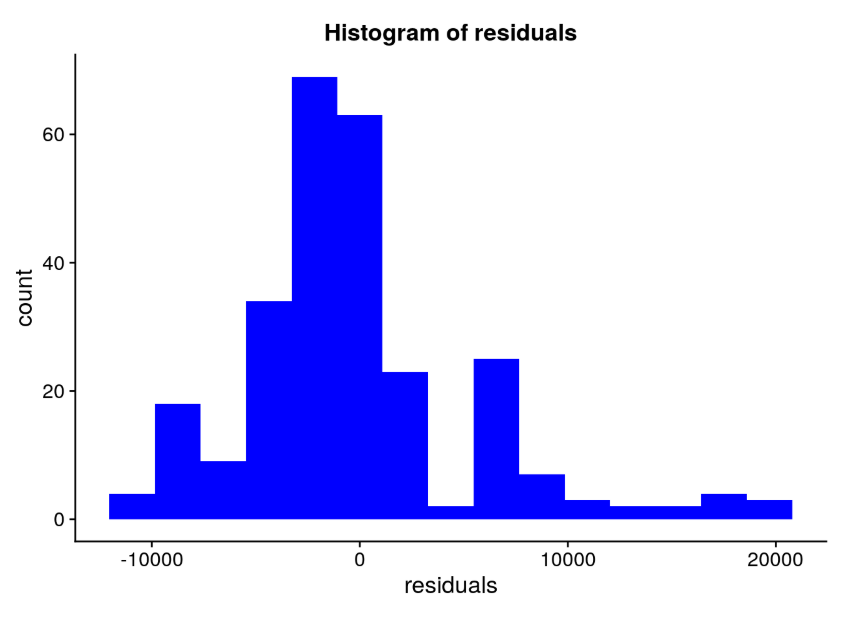
\includegraphics[width=8cm]{img/3.png}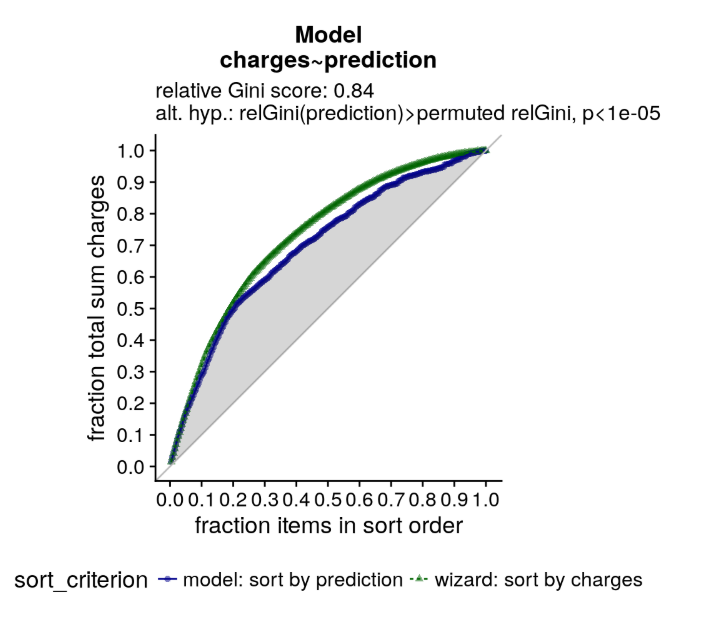
\includegraphics[width=8cm]{img/4.png}
\end{center}
As the graphs depict, the model predicts fairly well since most of the residuals allocate close to 0. However, as the prediction values increases, the residuals also varies slightly. But overall, the model still performed acceptably well. \\ \\
Finally, to confirm the model’s performance, some examples will be given to test the model. Three different people with different information will be given to see how much the Insurance charges on health care will be for each of them. \\ \\
\textbf{Person 1}: Nguyen Van A, 20 years old, BMI 25.4, no children, smokes, from northwest.
Health care charges for Nguyen Van A: 25235.4 \\
\textbf{Person 2}: Tran Duc B, 56 years old, BMI 49, 3 children, doesn’t smoke, from northeast.
Health care charges for Tran Duc B: 19904.57 \\
\textbf{Person 3}: Dang Van C, 30 years old, BMI 31.2, 1 children, smokes, from southeast.
Health care charges for Dang Van C: 29561.78
\subsubsection{The Result}
From the performance of our testing model and the results of the prediction shown above, “sex” attribute does not affect much on insurance charges, but being a smoker influences heavily on the amount of charge one person will be charged, which is satisfiable to our initial assumption. 
\newpage
\subsection{Two-way Analysis of Variance (ANOVA)}
\subsubsection{Definition}
\textbf{Analysis of variance} (ANOVA) is a statistical method that separates observed aggregate variability found inside a dataset into two basic components: dependent factors and independent factors. Analysts use the ANOVA test to determine the influence that independent variables have on the dependent variable in a regression study. The two-way ANOVA compares the mean differences between groups that have been split on two independent variables (called factors). The primary purpose of a two-way ANOVA is to understand if there is an interaction between the two independent variables on the dependent variable.
\subsubsection{Implementation}
\textbf{Hypothesis Representation}
In this statistical method,there are three null hypotheses we need to test:
\begin{itemize}
    \item There is no difference in the means of observations grouped by one factor 
    \item There is no difference in the means of observations grouped by the other factor
    \item There is no interaction between two factors
\end{itemize}
\textbf{Data preparation}
In order to conduct this method in R, we sample a group of 460 rows which have full attributes.In this study, we want to evaluate if there is a significant two-way interaction between sex and smoker factor on explaining the total charges. An interaction effect occurs when the effect of one independent variable on an outcome variable depends on the level of the other independent variables.
\subsubsection{Checking the validity of the test}
Since ANOVA assumes that the data are normally distributed and the variance across groups are homogeneous. We can check that with some diagnostic plots.\\ \\
\textbf{Normality plot of the residuals}. In the plot below, the quantiles of the residuals are plotted against the quantiles of the normal distribution. A 45-degree reference line is also plotted.\\ \\
The normal probability plot of residuals is used to verify the assumption that the residuals are normally distributed.\\ \\
The normal probability plot of the residuals should approximately follow a straight line.\\ \\
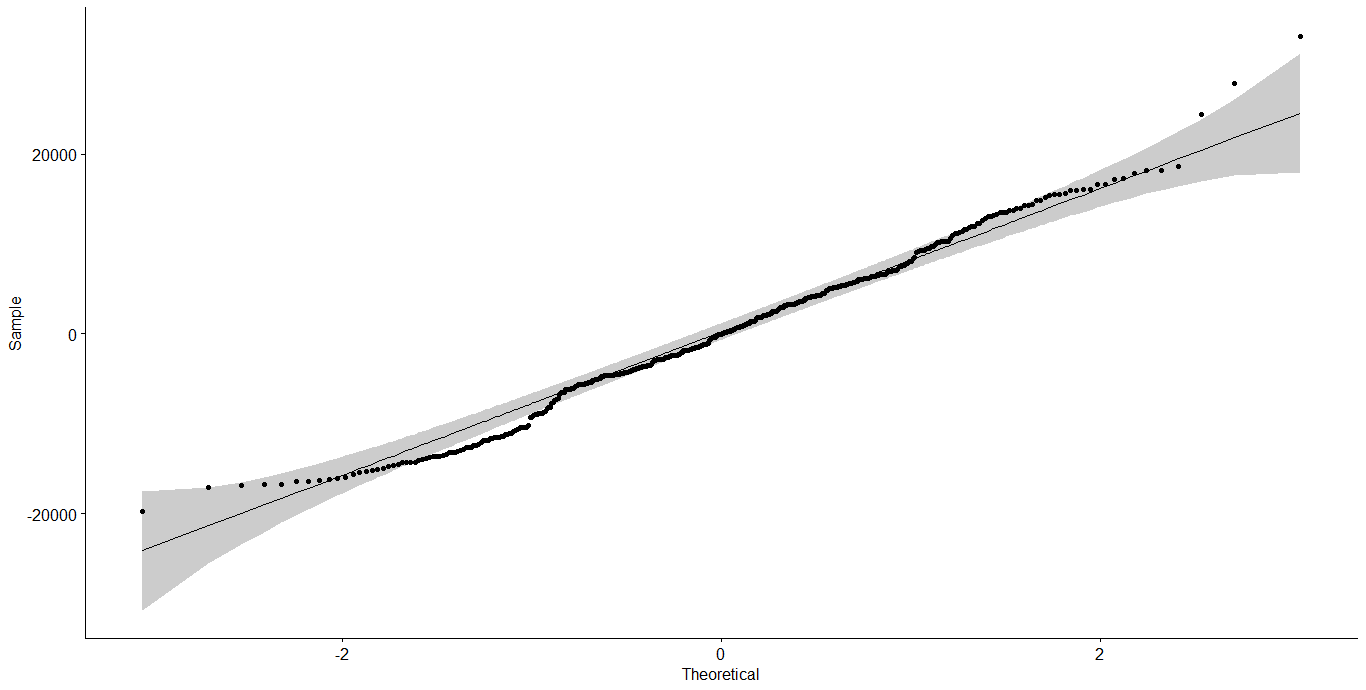
\includegraphics[width=14cm]{img/normality.png} \\ \\
As all the point follow a straight line, we can assume normality for our dataset. We do not conduct Shapiro-Wilk test(which is very popular when testing normality) because the sample size in this case is very big since for large amounts of data even very small deviations from normality can be detected, leading to rejection of the null hypothesis event though for practical purposes the data is more than normal enough. \\ \\
\textbf{Homogeneity check} \\ \\
The \textbf{residuals versus fits plot} is used to check the homogeneity of variances. In the plot below, there is no evident relationships between residuals and fitted values (the mean of each groups), which is very good. Linear property seems to hold reasonably well as the red line is close to the dashed line. Therefore we can assume the homogeneity of variances. \\
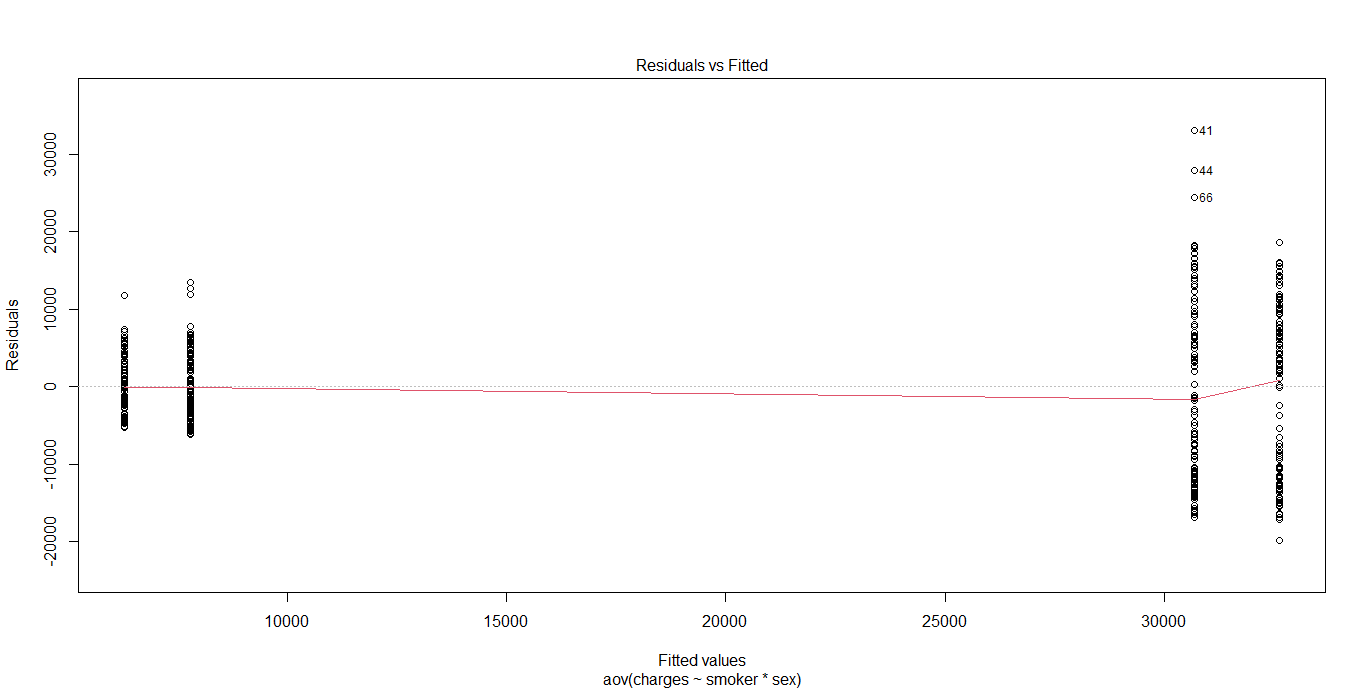
\includegraphics[width=15cm]{img/homogenity.png}
\subsubsection{Computation}
To comprehend the analysis of variance model, we create a model named modelaov by using function aov() in R studio. And then we fit the model in function Anova() with type “III” sums of squares. After computing, the program displays a table of information as above figure, each column with different value. \\ \\
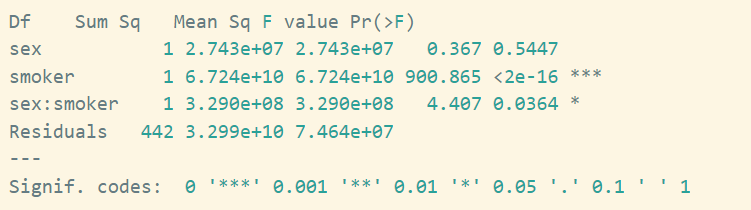
\includegraphics[width=14cm]{img/computation.png}
\begin{itemize}
    \item Sum Sq: These are the sum of squares for all rows.
    \item Df: This is the degrees of freedom. 
    \item F value: This is the F statistic associated with the given source. 
    \item Pr(>F): This is the p-value associated with the F statistic of a given source. 
\end{itemize}
\subsubsection{The Result}
A two-way ANOVA was conducted to examine the effects of sex and smoker on insurance charges. \\ \\
Residual analysis was performed to test for the assumptions of the two-way ANOVA. \\ \\
There were no extreme outliers, residuals were normally distributed and there was homogeneity of variances. \\ \\
From ANOVA table, we can conclude there was statistically significant interaction between sex and smoker on total insurance charges (p-value = 0.0364 < 0.05) which indicate that the relationships between “sex” and insurance charges depends on the smoker factor . “smoker” factor effect is statistically significant (p-value < 2*$10^{-16}$ ) while “sex”’s effect is very weak(p-value =0.5547). The result proves that whether the person is smoker or not will impact significantly the mean insurance charges.


%%%%%%%%%%%%%%%%%%%%%%%%%%%%%%%%%
%%%%%%%%%%%%%%%%%%%%%%%%%%%%%%%%%
\newpage
\section{Discussion and Conclusion}
Throughout the project, the main aim of our research is to understand the relationships between independent variables in a dataset by applying statistical data analysis methods. From the outcome of both methods (Linear Regression and ANOVA), it is evident that being a smoker, regardless of sex, will influence heavily on a person’s health and, therefore, results in a drastic increase in the personal medical charges. \\ \\
This study also found that there is a considerable increase in the cost of medical care as a person’s BMI record goes up. Hence, it is advisable that one stay in shape and try to keep their BMI in the optimal and healthy degree to assure a healthy lifestyle as well as to maintain their budget low as low as possible. \\ \\
One of the limitations of this study is that we selected R to perform the data analysis since, comparing to Python, R is much more complicated, which resulted in us taking more time than expected to do research about the language as well as browsing for suitable packages to graph the data suitably. Moreover, there are still much more to be improved in the way we access the data such as separating the data in to the smoker and non-smoker categories to do further analysis. Nevertheless, we still managed to graph the data in an easy-to-understand way and did the data analysis reasonably well. \\ \\
Bringing up the rear, this study provided evidence that a person should stay in his/her healthy shape as well as say no to smoking as a hobby to experience a better life.
%%%%%%%%%%%%%%%%%%%%%%%%%%%%%%%%%
\newpage
\begin{thebibliography}{80}

\bibitem{bib1}
{\em  Linear Regression Tutorial}, Kaggle,\\ 
{\color{blue}https://www.kaggle.com/sudhirnl7/linear-regression-tutorial}

\bibitem{bib2}
{\em Linear regression}, Wikipedia,\\
{\color{blue}https://en.wikipedia.org/wiki/Linear\_regression}

\bibitem{bib3}
{\em Health Care Cost Prediction w/ Linear Regression}, Kaggle,\\
{\color{blue}https://www.kaggle.com/ruslankl/health-care-cost-prediction-w-linear-regression}

\bibitem{bib4}
{\em Analysis of variance}, Wikipedia,\\
{\color{blue}https://en.wikipedia.org/wiki/Analysis\_of\_variance}

\bibitem{bib5}
{\em Two-way analysis of variance}, Wikipedia,\\
{\color{blue}https://en.wikipedia.org/wiki/Two-way\_analysis\_of\_variance}

\bibitem{bib6}
{\em Two-Way ANOVA Test in R}, STHDA,\\
{\color{blue}http://www.sthda.com/english/wiki/two-way-anova-test-in-r}
\end{thebibliography}   
\end{document}